\documentclass[twocolumn,a4j]{jarticle}

\usepackage{ascmac}
\usepackage{graphicx}
\usepackage{otf}
\usepackage{epsf}

%% 以下のスタイル情報は変更しない
\setlength{\textheight}{247mm}
\setlength{\textwidth}{160mm}
\setlength{\topmargin}{-19mm}
\setlength{\oddsidemargin}{0mm}

\title{Mashupによるe-learningコンテンツ検索システムの開発}   
\author{佐賀大学 理工学部 知能情報システム学科 第4研究グループ\\ 発表者:甲斐 \UTF{F9C3}馬 (08233014)\\ 指導教員:新井 康平 教授}

\begin{document}
\date{\empty}
\maketitle
\thispagestyle{empty}

\section{序論}
Mashupはポータルと同様にコンテンツ検索を可能にするツールであるが、Web2.0を用いてコンテンツを分類する、異なるサイトのAPIを利用する、クライアント・サーバー双方で検索ができる、検索は任意の構造化ハイブリッドコンテンツとして個々のコンテンツを混合して行える、XML変換のREST,RSS,Atom等が利用できるといった特徴がある。これらを利用し、既提案モデル納豆ビューによるコンテンツの三次元空間にノードグラフを展開して操作可能とするAndroid上での検索システムを構築した。

\section{先行研究}
\begin{figure}[htbp]
\begin{center}
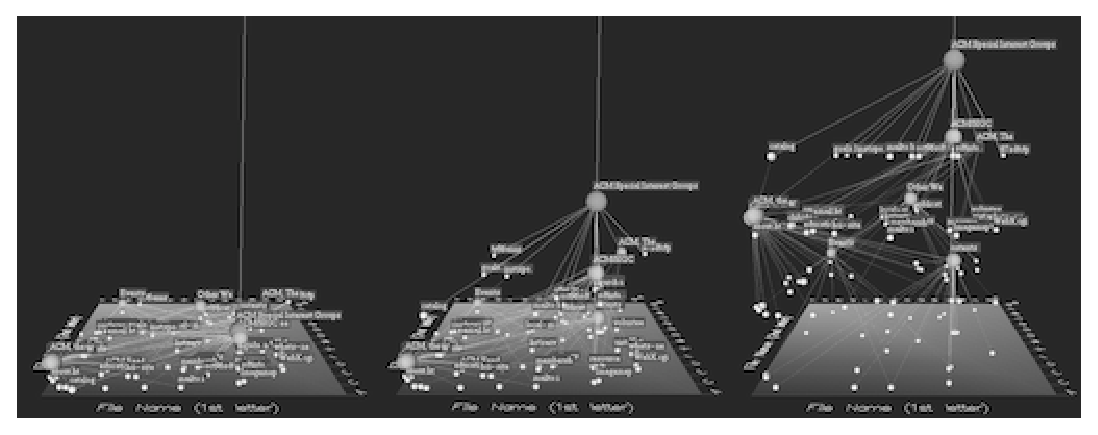
\includegraphics[width=7.5cm]{eps/natto-kuro.eps}
\caption{納豆ビューによる持ち上げ操作}
\label{natto}
\end{center}
\end{figure}
ノードグラフ型のWWW視覚化の一つとして、塩澤らによって開発された「納豆ビュー」\cite{natto}が存在する。このGUIでは、グラフ上に展開したノードをリンクに見立てており、サイト間のリンク関係がエッジで表示される。xy平面には一意的な座標が与えられ、z軸方向にはノードを摘んで持ち上げる、つまりユーザによる操作が可能となっている。これにより、複雑なネットワークをユーザの意志によってわかりやすく可視化することが可能になる。当研究ではこれらのデザインを参考に、一意的な意味付けを持つノードグラフ型のデザインを考えた。
\section{LEDOXEA}
\begin{figure}[htbp]
 \begin{minipage}{0.45\hsize}
  \begin{center}
   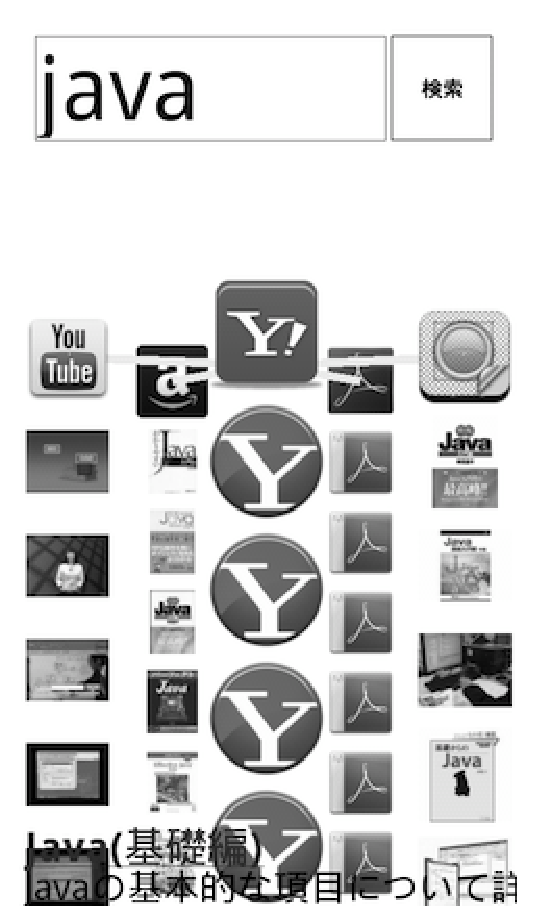
\includegraphics[width=20mm]{eps/ledoxea01.eps}
  \end{center}
  \caption{結果表示画面}
  \label{le01}
 \end{minipage}
 \begin{minipage}{0.45\hsize}
  \begin{center}
   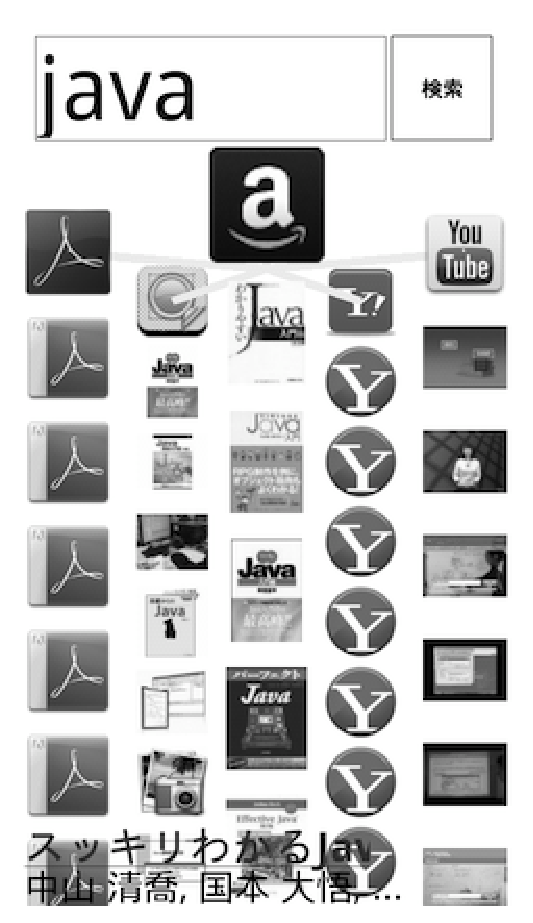
\includegraphics[width=20mm]{eps/ledoxea02.eps}
  \end{center}
  \caption{回転操作}
  \label{le02}
 \end{minipage}
\end{figure}
MashupによるAndroidスマートフォン向けのアプリ「LEDOXEA」を開発した。x-y平面に検索エンジン毎の検索結果を描画し、z軸方向に一定間隔で展開することによって、一意的な意味付けを持つ操作を可能なグラフ型のGUIを構築した。なお、e-learningコンテンツの検索に特化するため、昨年度研究成果\cite{docsearch}より、内部的に2種のサブキーワードをOR検索にて併用している。
\vspace{-5mm}
\section{評価,結論}
フィードバックの結果、検索結果の一覧性や、スワイプ動作の独特な動作による面白さを評価する意見があった。これにより当命題は満たせたと言える。今後の課題として、それぞれの検索結果をより深く融合して、特徴空間におけるコンテンツの特徴ベクトルに基づくシステムへ再構成し、よりシンプルに結果まで辿り着くようにすることが挙げられる。
\vspace{-5mm}
%% 参考文献を記述する。
\begin{thebibliography}{9}\setlength{\itemsep}{2ex}\small
\bibitem{natto} 塩澤秀和, 西山晴彦, 松下温:「納豆ビュー」の対話的 な情報視覚化における位置づけ,情報処理学会論文誌 Vol.38 No.11, pp.2331-2342, 1997.11.
\bibitem{docsearch} 原真琴:e-learningコンテンツにおけるドキュメントサーチの最適化,2012.3.

\end{thebibliography}
\end{document}
